\documentclass[a4paper,french,bookmarks]{article}
\usepackage{./Structure/4PE18TEXTB}

\begin{document}
\stylizeDoc{Physique}{Chapitre 20}{Le corps pur diphasé}

\initcours{}

{\sffamily \bfseries Note à un potentiel lecteur :} Bien que le cours ci-dessous soit principalement basé sur celui qui m'a été donné, j'y ai également incorporé quelques informations que j'ai pu trouver ailleurs, généralement sur internet. Ce document ne devrait \textit{a priori} servir qu'à ma personne, mais dans le cas où il serait partagé, j'aviserai tout lecteur à re-vérifier lui-même les contenus sur lesquels il a un doute.

\section{Corps pur sous différentes phases}

\subsection{Notion de phase}

Ce deuxième chapitre de thermodynamique porte sur les corps pur diphasés. On commence donc par définir le concept de \guill{phase}, qui recoupe la notion plus familière d'état de la matière (solide, liquide, gazeux) abordée plus tôt dans le cursus. Si l'on a aisément une conception intuitive des états de la matière (solide, liquide, gazeux, \dots) et donc des phases, il ne semble pas tout aussi de donner une définition rigoureuse.

\begin{enumerate}
    \itt Certains ouvrages ont une approche plus \guill{substantielle}, consistant grossièrement à considérer qu'une phase d'un système thermodynamique est une des parties homogène de ce système ;
    
    \itt d'autres préfèrent une approche plus \guill{analytique}, consistant à considérer une phase comme un domaine de stabilité, c'est-à-dire où les paramètres varient de manière continue. C'est la définition qu'on retient ici :
\end{enumerate} 

\begin{definition}{Phase}{}
    On dit qu'un sous-ensemble d'un système thermodynamique est une \hg{phase} lorsque les \hg{variables intensives} y \hg{varient continûment}.
\end{definition}

On peut donc distinguer les différentes phases d'un système thermodynamique en y repérant des discontinuités. On donne ci-dessous des exemples de systèmes thermodynamiques comprenant plusieurs phases :

\begin{example}{}{}
    \begin{enumerate}
        \begin{minipage}{0.5\linewidth}
            \itt Verre d'eau avec un glaçon
            
            \begin{center}
                \begin{tikzpicture}
                    \draw[] (0, -2) arc (360:180:-0.5 and -0.1) -- (1, -2);
                    
                    \draw[] (0, 0) arc (360:180:-0.5 and -0.1) -- (1, 0);
                    
                    \draw[black!50] (0.5, -1.25) -- (1.5, -1.25) node[right] {{\color{main1!70} Eau} (phase liquide)};
                    
                    \draw[draw=none, fill=main1!30] (0.35, -0.45) -- (0.35, -0.7) -- (0.65, -0.7) -- (0.65, -0.45) -- (0.35, -0.45);
                    
                    \draw[top color=main2!15,bottom color=main2!50,opacity=0.7,draw=none] (0, -0.5) -- (0, -2) arc (360:180:-0.5 and 0.1) -- (1, -2) -- (1, -0.5);
                    
                    \draw[white, fill=main2!30] (0, -0.5) arc (360:180:-0.5 and -0.1) -- (1, -0.5) arc (360:180:0.5 and 0.1) -- (0, -0.5);
                    
                    \draw[black!50] (0.5, -0.47) -- (1.5, -0.47) node[right] {{\color{main2!80} Glaçon} (phase solide)};
                    
                    \draw[draw=none, fill=main1!10] (0.35, -0.45) -- (0.35, -0.55) arc (360:180:-0.15 and 0.02) -- (0.65, -0.55) -- (0.65, -0.45) -- (0.35, -0.45);
                    
                    \draw[white, thin] (0.2, -0.5) arc (360:180:-0.3 and 0.06) -- (0.8, -0.5);
                    
                    \draw[draw=none, fill=main1!25] (0.35, -0.45) -- (0.36, -0.40) -- (0.64, -0.40) -- (0.65, -0.45) -- (0.35, -0.45);
                    
                    \draw[] (0, 0) -- (0, -2) arc (360:180:-0.5 and 0.1) -- (1, -2) -- (1, 0) arc (360:180:0.5 and 0.1) -- (0, 0);
                \end{tikzpicture}
            \end{center}
        \end{minipage}
        \begin{minipage}{0.5\linewidth}
            \itt Huile et eau (discontinuité de $\rho$)
            
            \begin{center}
                \begin{tikzpicture}
                    \draw[] (0, -2) arc (360:180:-0.5 and -0.1) -- (1, -2);
                    
                    \draw[] (0, 0) arc (360:180:-0.5 and -0.1) -- (1, 0);
                    
                    \draw[black!50] (0.5, -1.25) -- (1.5, -1.25) node[right] {{\color{main1!70} Eau} (phase liquide)};
                    
                    \draw[top color=main2!15,bottom color=main2!50,opacity=0.7,draw=white] (0, -0.5) -- (0, -2) arc (360:180:-0.5 and 0.1) -- (1, -2) -- (1, -0.5) arc (360:180:0.5 and 0.1) -- (0, -0.5);
                    
                    \draw[white, fill=main2!30, opacity=0.3] (0, -0.5) arc (360:180:-0.5 and -0.1) -- (1, -0.5) arc (360:180:0.5 and 0.1) -- (0, -0.5);
                    
                    \draw[white] (0, -0.5) arc (360:180:-0.5 and -0.1) -- (1, -0.5);
                    
                    \draw[black!50] (0.5, -0.45) -- (1.5, -0.45) node[right] {{\color{yellow!50!orange} Huile} (phase liquide)};
                    
                    \draw[top color=yellow!50!orange!15,bottom color=yellow!50!orange!50,opacity=0.7,draw=none] (0, -0.3) -- (0, -0.5) arc (360:180:-0.5 and 0.1) -- (1, -0.5) -- (1, -0.3);

                    \draw[white, fill=yellow!50!orange!30] (0, -0.3) arc (360:180:-0.5 and -0.1) -- (1, -0.3) arc (360:180:0.5 and 0.1) -- (0, -0.3);
                    
                    \draw[] (0, 0) -- (0, -2) arc (360:180:-0.5 and 0.1) -- (1, -2) -- (1, 0) arc (360:180:0.5 and 0.1) -- (0, 0);
                \end{tikzpicture}
            \end{center}
        \end{minipage}
        
        \itt Si considérée, l'atmosphère représente dans les deux exemples ci-dessus une phase gazeuse.
    \end{enumerate}
\end{example}

On introduit une terminologie particulière pour désigner le nombre de phases d'un système thermodynamique :

\begin{definition}{Système monophasé, diphasé et triphasé}{}
    Un système thermodynamique est dit
    %
    \begin{enumerate}
        \ithand \hg{monophasé} lorsqu'il \hg{comprend 1 phase} ;
        \ithand \hg{diphasé} lorsqu'il \hg{comprend 2 phases} ;
        \ithand \hg{triphasé} lorsqu'il \hg{comprend 3 phases}.
    \end{enumerate}
\end{definition}

Les systèmes thermodynamiques monophasés ont été étudiés au chapitre 19. Les systèmes thermodynamiques diphasés et triphasés seront étudiés dans les chapitres 20 et 21. On définit également la notion de corps pur :

\begin{definition}{Corps pur}{}
    On dit qu'un corps est un \hg{corps pur} lorsqu'il n'est composé que d'\hg{une seule espèce chimique}.
\end{definition}

Dans la suite, on considère un corps pur diphasé. On donne ci dessous les noms des transitions de phases entre les états liquides, solides et gazeux :

\begin{definition}{Transitions de phase}{}
    \begin{enumerate}
        \ithand La transition de phase de l'état \hg{solide à liquide} est la \hg{fusion} ;
        
        \ithand La transition de phase de l'état \hg{liquide à solide} est la \hg{solidification} ;
        
        \ithand La transition de phase de l'état \hg{solide à gazeux} est la \hg{sublimation} ;
        
        \ithand La transition de phase de l'état \hg{gazeux à solide} est la \hg{condensation} ;
        
        \ithand La transition de phase de l'état \hg{liquide à gazeux} est la \hg{vaporisation} ;
        
        \ithand La transition de phase de l'état \hg{gazeux à solide} est la \hg{liquéfaction}.
    \end{enumerate}
\end{definition}

\begin{center}
    \begin{tikzpicture}
        \node[rectangle,inner sep=7pt] (G) at (0, 3) {\phantom{\large Vapeur / Gaz}};
        \node[rectangle,inner sep=7pt] (S) at (-2.9, -1.5) {\phantom{\large Solide}};
        \node[rectangle,inner sep=7pt] (L) at (2.9, -1.5) {\phantom{\large Liquide}};
        
        %\node[rectangle,fill=main7,opacity=0.2] at (-2.9, -1.5) {\phantom{K}};
        
        %\foreach \point in {1,...,4}{
        %    \pgfmathparse{random()}
        %    \pgfmathsetmacro\xpos{2*\pgfmathresult}
        %    \pgfmathparse{random()}
        %    \pgfmathsetmacro\ypos{1*\pgfmathresult}
        %    \pgfmathrandom{0.1,1}
        %    \let\pointwidth\pgfmathresult
        %    \node[rectangle,inner sep=\pointwidth pt,fill=main7,opacity=0.2] at %(-3.9+\xpos,-2+\ypos) {\phantom{\tiny .}};
        %}
        
        %\foreach \point in {1,...,4}{
        %    \pgfmathparse{random()}
        %    \pgfmathsetmacro\xpos{2*\pgfmathresult}
        %    \pgfmathparse{random()}
        %    \pgfmathsetmacro\ypos{1*\pgfmathresult}
        %    \pgfmathrandom{0.1,1}
        %    \let\pointwidth\pgfmathresult
        %    \node[circle,inner sep=\pointwidth pt,fill=main1,opacity=0.2] at %(1.9+\xpos,-2+\ypos) {\phantom{\tiny .}};
        %}
        
        %\foreach \point in {1,...,4}{
        %    \pgfmathparse{random()}
        %    \pgfmathsetmacro\xpos{3*\pgfmathresult}
        %    \pgfmathparse{random()}
        %    \pgfmathsetmacro\ypos{1*\pgfmathresult}
        %    \node[opacity=0.3] at (-1.5+\xpos,2.4+\ypos) {$\color{main5} %\widetilde{\phantom{oio}}$};
        %}
        
        \node[rectangle,fill=main4!50,opacity=0.5] at (0, 3) {\phantom{\large Vapeur / Gaz}};
        \node[rectangle,fill=main7!50,opacity=0.5] at (-2.9, -1.5) {\phantom{\large  Solide}};
        \node[rectangle,fill=main1!50,opacity=0.5] at (2.9, -1.5) {\phantom{\large Liquide}};
        
        \node[rectangle] at (0, 3) {\large\color{main4} Vapeur / Gaz};
        \node[rectangle] at (-2.9, -1.5) {\large\color{main7} Solide};
        \node[rectangle] at (2.9, -1.5) {\large\color{main1} Liquide};
        
        \draw[gradientdraw={0.3pt}{main4}{main7}, ->, main7] ([yshift=-4pt]G.west) to [bend left=20] node [sloped, anchor=center, below] {Condensation} (S.north);
        
        \draw[gradientdraw={0.3pt}{main7}{main4}, ->, main4] ([xshift=-4pt]S.north) to [bend left=20] node [sloped, anchor=center, above] {Sublimation} (G.west);
        
        \draw[gradientdraw={0.3pt}{main7}{main1}, ->, main1] ([yshift=-4pt]S.east) to [bend right=20] node [sloped, anchor=center, below] {Fusion} (L.west);
        
        \draw[gradientdraw={0.3pt}{main1}{main7}, ->, main7] ([yshift=4pt]L.west) to [bend right=20] node [sloped, anchor=center, above] {Solidification} (S.east);
        
        \draw[gradientdraw={0.3pt}{main1}{main4}, ->, main4] ([xshift=4pt]L.north) to [bend right=20] node [sloped, anchor=center, above] {Vaporisation} (G.east);
        
        \draw[gradientdraw={0.3pt}{main4}{main1}, ->, main1] ([yshift=-4pt]G.east) to [bend right=20] node [sloped, anchor=center, below] {Liquéfaction} (L.north);
    \end{tikzpicture}
\end{center}

\subsection{Diagramme de phase d'un corps pur}

L'état d'une phase dépend de certain paramètres : l'eau par exemple, devient solide aux alentours des \SI{0}{\celsius} et boue (se vaporise) aux alentours des \SI{100}{\celsius}. Pour situer les différents états d'un système thermodynamique en fonctions des paramètres, on peut notamment utiliser des diagrammes de phase :

\begin{definition}{Diagramme de phase}{}
    On appelle \hg{diagramme de phase} la \hg{représentation graphique de l'état d'un système thermodynamique} en fonction de \hg{deux variables d'état}. 
\end{definition}

\begin{minipage}{0.45\linewidth}
    \begin{center}
        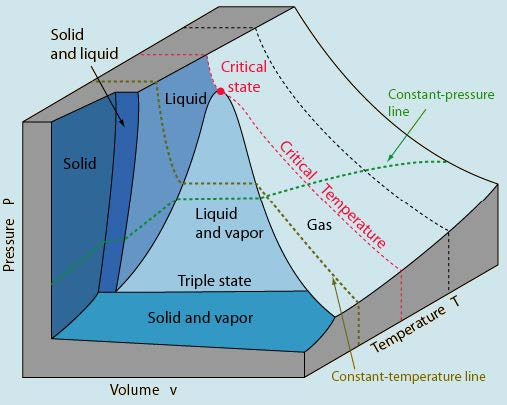
\includegraphics[scale=0.77]{Physique/Cours/chap20fig/fig_1.jpg}
    \end{center}
\end{minipage}
%
\hfill
%
\begin{minipage}{0.5\linewidth}
    Un système thermodynamique dépendant de trois variables d'état ($P$, $T$ et $V$), il s'agit donc de la projection à deux dimension d'une surface qui vit dans un graphe à trois dimensions, comme représenté ci-contre. Chaque point de cette surface correspond à un état d'équilibre. Les variables sont ainsi liées : on ne pourra jamais \guill{sortir} de cette surface.\\
    
    {\sffamily \bfseries NB :} Dans la représentation ci-contre, $v$ désigne le volume massique, à savoir le volume $V$ divisé par la masse $m$.
\end{minipage}

\subsection{Premier exemple : Le diagramme (P, T)}

On étudie un premier exemple de diagramme de phase : le diagramme $(P, T)$.

\begin{definition}{Diagramme (P, T)}{}
    On appelle \hg{diagramme $(P, T)$} le \hg{diagramme de phase} en fonction de $P$ en ordonnée et $T$ en abscisse.
\end{definition}

Le diagramme $(P, T)$ est donc une projection le long de l'axe $V$. En conséquence, on ne peut y trouver d'information sur $V$.

\subsubsection{Lecture du diagramme}

Le tracé qualitatif du diagramme $(P, T)$ doit être connu. On le donne ci-dessous dans le cas d'un corps pur quelconque et dans le cas particulier de l'eau.\medskip

\begin{minipage}{0.48\linewidth}
    \begin{center}
        \underline{Corps pur quelconque}\\[3pt]
        
        \begin{tikzpicture}
            \begin{axis}[
                axis lines = left,
                axis line style={thick axis arrow},
                xlabel=$T$,
                ylabel=$P$,
                xlabel style = {at={(axis description cs:1,0)},anchor=north east},
                ylabel style = {at={(axis description cs:0,1)},anchor=north east,rotate=-90},
                domain=0:10,
                xmin=0,
                xmax=12,
                ymin=0,
                ymax=10,
                ticks=none,
                grid = none,
                axis on top
            ]
            
            \coordinate (O) at (0,0.5);
            \coordinate (N1) at (5,10);
            \coordinate (N2) at (11,10);
            \coordinate (NE) at (12,10);
            \coordinate (NW) at (0,10);
            \coordinate (SE) at (12,0);
            \coordinate (SW) at (0, 0);
            \coordinate (W) at (0,5);
            \coordinate (S) at (6,0);
            \coordinate (C) at (10.2,7.8); % critical
            \coordinate (T) at (4,3); % triple
            
            % CHEMINS
            \def\SL{(T) -- (N1)}
            \def\SG{(O) to[out=20,in=-120] (T)}
            \def\LG{(T) to[out=20,in=-120] (C)}
            \def\atm{(0,5.5) -- (12,5.5)}
            \path[name path=SL] \SL;
            \path[name path=LG] \LG;
            \path[name path=atm] \atm;
            
            % REGIONS
            \fill[main7!20] \SG -- (N1) -- (NW) -- cycle;
            \fill[main1!20] \LG -- (N2) -- (N1) -- cycle;
            \fill[main4!20] \LG -- (N2) -- (NE) -- (SE) -- (SW) -- \SG -- cycle;
            \node at (2,5) {\color{main7} Solide (S)};
            \node at (8,2.2) {\color{main4} Vapeur / Gaz (G)};
            \node at (6.5,6.6) {\color{main1} Liquide (L)};
            
            %LIGNES
            \draw[thick] \SG;
            \draw[thick] \LG;
            \draw[thick] \SL;
            
            % POINTS
            \fill[] (C) circle (1.5pt) node[above=1pt,scale=0.6,align=center] {C};
            \fill[main10] (T) circle (3pt) node[below right,main10,scale=0.9,align=right] {\textsc{iii}};
        \end{axis}
    \end{tikzpicture}
    \end{center}
\end{minipage}
%
\hfill
%
\begin{minipage}{0.48\linewidth}
    \begin{center}
        \underline{Cas de l'eau}\\[3pt]
        
        \begin{tikzpicture}
            \begin{axis}[
                axis lines = left,
                axis line style={thick axis arrow},
                xlabel=$T$,
                ylabel=$P$,
                xlabel style = {at={(axis description cs:1,0)},anchor=north east},
                ylabel style = {at={(axis description cs:0,1)},anchor=north east,rotate=-90},
                domain=0:10,
                xmin=0,
                xmax=12,
                ymin=0,
                ymax=10,
                ticks=none,
                grid = none,
                axis on top
            ]
            
            \coordinate (O) at (0,0.5);
            \coordinate (N1) at (3,10);
            \coordinate (N2) at (11,10);
            \coordinate (NE) at (12,10);
            \coordinate (NW) at (0,10);
            \coordinate (SE) at (12,0);
            \coordinate (SW) at (0, 0);
            \coordinate (W) at (0,5);
            \coordinate (S) at (6,0);
            \coordinate (C) at (10.2,7.8); % critical
            \coordinate (T) at (4,3); % triple
            
            % CHEMINS
            \def\SL{(T) -- (N1)}
            \def\SG{(O) to[out=20,in=-120] (T)}
            \def\LG{(T) to[out=20,in=-120] (C)}
            \def\atm{(0,5.5) -- (12,5.5)}
            \path[name path=SL] \SL;
            \path[name path=LG] \LG;
            \path[name path=atm] \atm;
            
            % REGIONS
            \fill[main7!20] \SG -- (N1) -- (NW) -- cycle;
            \fill[main1!20] \LG -- (N2) -- (N1) -- cycle;
            \fill[main4!20] (0, 0) -- \LG -- (N2) -- (NE) -- (SE) -- (SW) -- \SG -- cycle;
            \node at (2,5) {\color{main7} Solide (S)};
            \node at (8,2.2) {\color{main4} Vapeur / Gaz (G)};
            \node at (6,6.6) {\color{main1} Liquide (L)};
            
            %LIGNES
            \draw[thick] \SG;
            \draw[thick] \LG;
            \draw[thick] \SL;
            
            % POINTS
            \fill[] (C) circle (1.5pt) node[above=1pt,scale=0.6,align=center] {C};
            \fill[main10] (T) circle (3pt) node[below right,main10,scale=0.9,align=right] {\textsc{iii}};
        \end{axis}
    \end{tikzpicture}
    \end{center}
\end{minipage}

\text{}\medskip

On remarque que, contrairement à un corps pur quelconque, la pente de la frontière liquide-solide pour l'eau est de signe négatif. Ainsi, pour une certaine température (donc sur une même abscisse), la pression est plus élevée à l'état liquide qu'à l'état solide. Ceci explique notamment pourquoi un glaçon flotte, pourquoi un patineur glisse sur un ses patins (à glace), ou pourquoi le fond des océans ne gèlent pas.

Les lignes noires entre les différents états représentes des positions où coexistent deux phases. Passer une telle ligne revient à une \textit{transition de phase}. On repère également deux points particuliers :
%
\begin{enumerate}
    \itt Le point triple (noté {\color{main10} \textsc{iii}}) : solide, liquide et gaz y sont à l'équilibre. Pour l'eau, on a les valeurs de température et de pression du point triple suivantes :
    %
    \[ T_\textsc{iii} = \SI{273.16}{\kelvin} = \SI{0.01}{\celsius} \qquad\et\qquad P_\textsc{iii} = \SI{6.11e-3}{\bar}\]
    
    \itt Le point critique (noté $C$) : pour les températures supérieures à celles de ce point, il n'y a plus de distinction entre phase liquide et gazeuse. On parle alors de \textit{fluide hypercritique}. Pour l'eau, on a les valeurs de température et de pression du point critique suivantes :
    %
    \[ T_\text{C} = \SI{647}{\kelvin} \qquad\et\qquad P_\text{C} = \SI{221}{\bar}\]
\end{enumerate}

\begin{minipage}{0.48\linewidth}
    On précisera qu'un solide peut présenter plusieurs configurations, et qu'un corps peur exister sous différentes formes moléculaires ou cristallines. On parle en fait de \textit{variétés allotropiques}. Le graphite et le diamant sont par exemples deux variétés allotropiques du carbone. Ces différences de variétés peuvent être visibles sur le diagramme de phase. On donne ci-contre l'exemple du diagramme de phase du carbone, où l'on voit les domaines du diamant et du graphite.
\end{minipage}
%
\hfill
%
\begin{minipage}{0.48\linewidth}
    \centering
    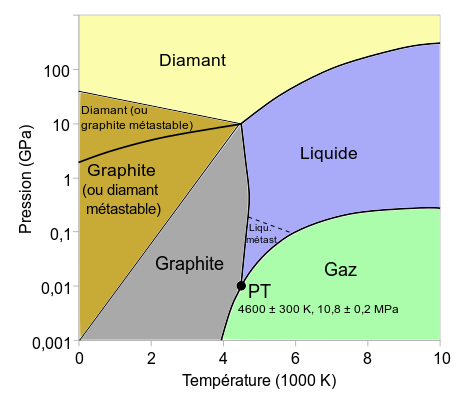
\includegraphics[scale=0.47]{Physique/Cours/chap20fig/fig_2.png}
\end{minipage}

\subsubsection{Condition de coexistence}

\begin{minipage}{0.58\linewidth}
    \centering
    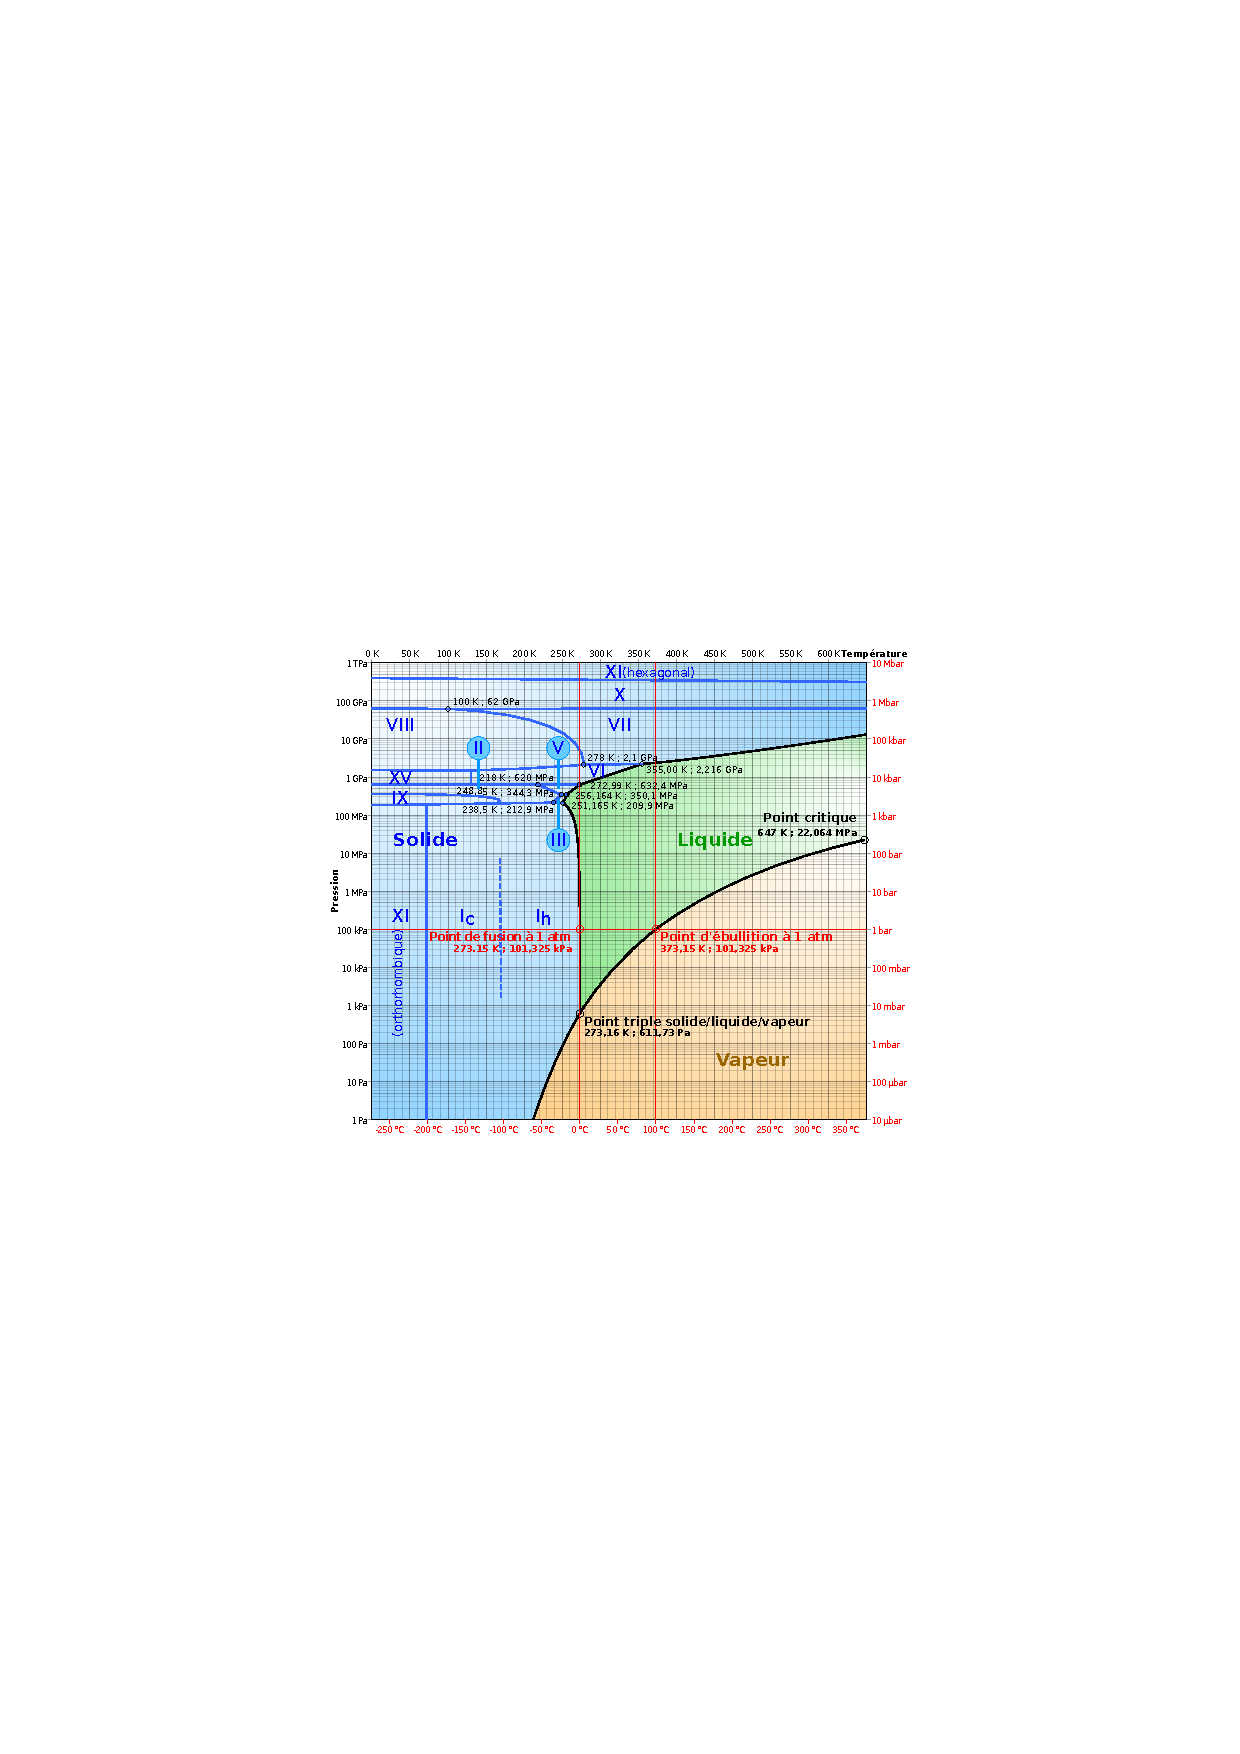
\includegraphics[]{Physique/Cours/chap20fig/fig_3.pdf}
\end{minipage}
%
\hfill
%
\begin{minipage}{0.4\linewidth}
    Lorsqu'un corps est à l'équilibre, sous deux phases $A$ et $B$, on se situe forcément sur une des \guill{lignes noires} introduites plus haut. La pression $P$ et la température sont ainsi liés, et en modélisant la \guill{ligne noire} en question dans le diagramme $(P, T)$ par une fonction $P_\text{AB}$, on a :
    %
    \[ P = P_\text{AB}\left(T\right)\]
    
    Pour une pression $P$ donné, il n'existe donc qu'une seule température $T$ à laquelle $A$ et $B$ sont à l'équilibre. On donne en exemples les valeurs ci-dessous, déjà connues de tous  :
    %
    \begin{enumerate}
        \itt pour $P = \SI{1}{\bar}$, l'eau liquide et solide sont en équilibre à $T = \SI{0}{\celsius}$ ;
        
        \itt pour $P = \SI{1}{\bar}$, l'eau liquide et gazeuse sont en équilibre à $T = \SI{100}{\celsius}$.
    \end{enumerate}
    %
    On donne en fait à $P_\text{LG}$ (pression de l'équilibre liquide-gaz / liquide vapeur) un nom particulier :
\end{minipage}

\begin{definition}{Pression de vapeur saturante}{}
    On appelle \hg{pression de vapeur saturante} la \hg{pression à laquelle la phase gazeuse est en équilibre avec la phase liquide}, en fonction de la température.
\end{definition}

La pression de vapeur saturante est généralement notée $P_\text{sat}\left(T\right) = P_\text{LG}\left(T\right)$.

\begin{enumerate}
    \itt Pour l'eau, on a $P_\text{sat}\left(\SI{100}{\celsius}\right) = \SI{1}{\bar}$.
\end{enumerate}

On ajoutera que tout cela implique l'existence d'un \textit{point} triple et pas d'une \textit{ligne} triple.

\subsubsection{En présence d'atmosphère inerte}

\begin{minipage}{0.48\linewidth}
    \begin{example}{}{}
        \underline{Verre d'eau}\medskip
        
        \begin{center}
            \begin{tikzpicture}
                \draw[] (0, -2) arc (360:180:-0.5 and -0.1) -- (1, -2);
                    
                \draw[] (0, 0) arc (360:180:-0.5 and -0.1) -- (1, 0);
                    
                \draw[black!50] (0.5, -1.25) -- (1.5, -1.25) node[right] {{\color{main1!70} Eau}};
                    
                \draw[top color=main2!15,bottom color=main2!50,opacity=0.7,draw=none] (0, -0.5) -- (0, -2) arc (360:180:-0.5 and 0.1) -- (1, -2) -- (1, -0.5);
                    
                \draw[white, fill=main2!30] (0, -0.5) arc (360:180:-0.5 and -0.1) -- (1, -0.5) arc (360:180:0.5 and 0.1) -- (0, -0.5);
                    
                \draw[] (0, 0) -- (0, -2) arc (360:180:-0.5 and 0.1) -- (1, -2) -- (1, 0) arc (360:180:0.5 and 0.1) -- (0, 0);
            \end{tikzpicture}
        \end{center}
    \end{example}
\end{minipage}
%
\hfill
%
\begin{minipage}{0.48\linewidth}
    Par \guill{inerte}, on entends \texit{qui ne joue pas de rôle chimique}.
\end{minipage}

\section{Etude détaillée de l'équilibre liquide-vapeur}

\subsection{Diagramme de Clapeyron}

\subsection{Stockage des fluides}



\end{document}